\documentclass[ignorenonframetext,]{beamer}
\setbeamertemplate{caption}[numbered]
\setbeamertemplate{caption label separator}{: }
\setbeamercolor{caption name}{fg=normal text.fg}
\beamertemplatenavigationsymbolsempty
\usepackage{lmodern}
\usepackage{amssymb,amsmath}
\usepackage{ifxetex,ifluatex}
\usepackage{fixltx2e} % provides \textsubscript
\ifnum 0\ifxetex 1\fi\ifluatex 1\fi=0 % if pdftex
  \usepackage[T1]{fontenc}
  \usepackage[utf8]{inputenc}
\else % if luatex or xelatex
  \ifxetex
    \usepackage{mathspec}
  \else
    \usepackage{fontspec}
  \fi
  \defaultfontfeatures{Ligatures=TeX,Scale=MatchLowercase}
\fi
% use upquote if available, for straight quotes in verbatim environments
\IfFileExists{upquote.sty}{\usepackage{upquote}}{}
% use microtype if available
\IfFileExists{microtype.sty}{%
\usepackage{microtype}
\UseMicrotypeSet[protrusion]{basicmath} % disable protrusion for tt fonts
}{}
\newif\ifbibliography
\hypersetup{
            pdftitle={Two Hidden Road Mortality Factors: Infrastructure Spending and Vehicle Safety Standards},
            pdfauthor={Ali Al-Ghaithi, Matthew Pelz, Xuan-Ha Vandenberg},
            pdfborder={0 0 0},
            breaklinks=true}
\urlstyle{same}  % don't use monospace font for urls
\usepackage{longtable,booktabs}
\usepackage{caption}
% These lines are needed to make table captions work with longtable:
\makeatletter
\def\fnum@table{\tablename~\thetable}
\makeatother
\usepackage{graphicx,grffile}
\makeatletter
\def\maxwidth{\ifdim\Gin@nat@width>\linewidth\linewidth\else\Gin@nat@width\fi}
\def\maxheight{\ifdim\Gin@nat@height>\textheight0.8\textheight\else\Gin@nat@height\fi}
\makeatother
% Scale images if necessary, so that they will not overflow the page
% margins by default, and it is still possible to overwrite the defaults
% using explicit options in \includegraphics[width, height, ...]{}
\setkeys{Gin}{width=\maxwidth,height=\maxheight,keepaspectratio}

% Prevent slide breaks in the middle of a paragraph:
\widowpenalties 1 10000
\raggedbottom

\AtBeginPart{
  \let\insertpartnumber\relax
  \let\partname\relax
  \frame{\partpage}
}
\AtBeginSection{
  \ifbibliography
  \else
    \let\insertsectionnumber\relax
    \let\sectionname\relax
    \frame{\sectionpage}
  \fi
}
\AtBeginSubsection{
  \let\insertsubsectionnumber\relax
  \let\subsectionname\relax
  \frame{\subsectionpage}
}

\setlength{\parindent}{0pt}
\setlength{\parskip}{6pt plus 2pt minus 1pt}
\setlength{\emergencystretch}{3em}  % prevent overfull lines
\providecommand{\tightlist}{%
  \setlength{\itemsep}{0pt}\setlength{\parskip}{0pt}}
\setcounter{secnumdepth}{0}

\title{Two Hidden Road Mortality Factors: Infrastructure Spending and Vehicle
Safety Standards}
\author{Ali Al-Ghaithi, Matthew Pelz, Xuan-Ha Vandenberg}
\date{12/12/2018}

\begin{document}
\frame{\titlepage}

\begin{frame}

\end{frame}

\begin{frame}{}

\begin{figure}
\centering
\includegraphics{Driving-in-oman.jpg}
\caption{}
\end{figure}

\begin{figure}
\centering
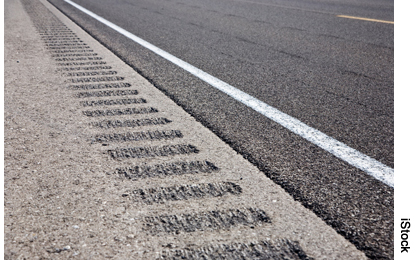
\includegraphics{EzZPb.jpg}
\caption{}
\end{figure}

\end{frame}

\begin{frame}{}

\begin{figure}
\centering
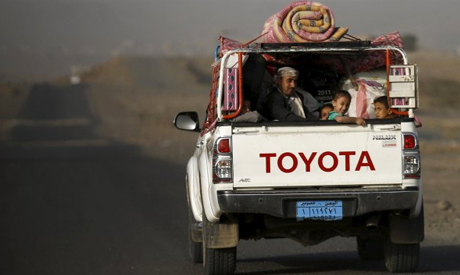
\includegraphics{road.jpg}
\caption{}
\end{figure}

\end{frame}

\begin{frame}{Studied Factors in Road Mortalities}

\begin{itemize}
\tightlist
\item
  {[}1{]} Speed Limits
\item
  {[}2{]} Vehicle Safety Standards
\item
  {[}3{]} Infrastructure Spending
\item
  {[}4{]} Traffic Congestion
\end{itemize}

\end{frame}

\begin{frame}{Figure 1: A subset of the Road Mortality Factors dataframe
created for the project and used during analysis.}

\begin{longtable}[]{@{}lrrrrr@{}}
\toprule
& rural & aggregate & roadspending & congestion &
deathsper100k\tabularnewline
\midrule
\endhead
afghanistan & 90 & 0 & NA & NA & 15.5\tabularnewline
albania & 80 & 0 & 107 & 0.3008905 & 15.1\tabularnewline
algeria & 100 & 0 & NA & NA & 23.8\tabularnewline
andorra & 90 & 7 & NA & NA & 7.6\tabularnewline
angola & 90 & 0 & NA & NA & 26.9\tabularnewline
antiguaandbarbuda & 64 & 0 & NA & NA & 6.7\tabularnewline
\bottomrule
\end{longtable}

\end{frame}

\begin{frame}{Linear Model}

\begin{center}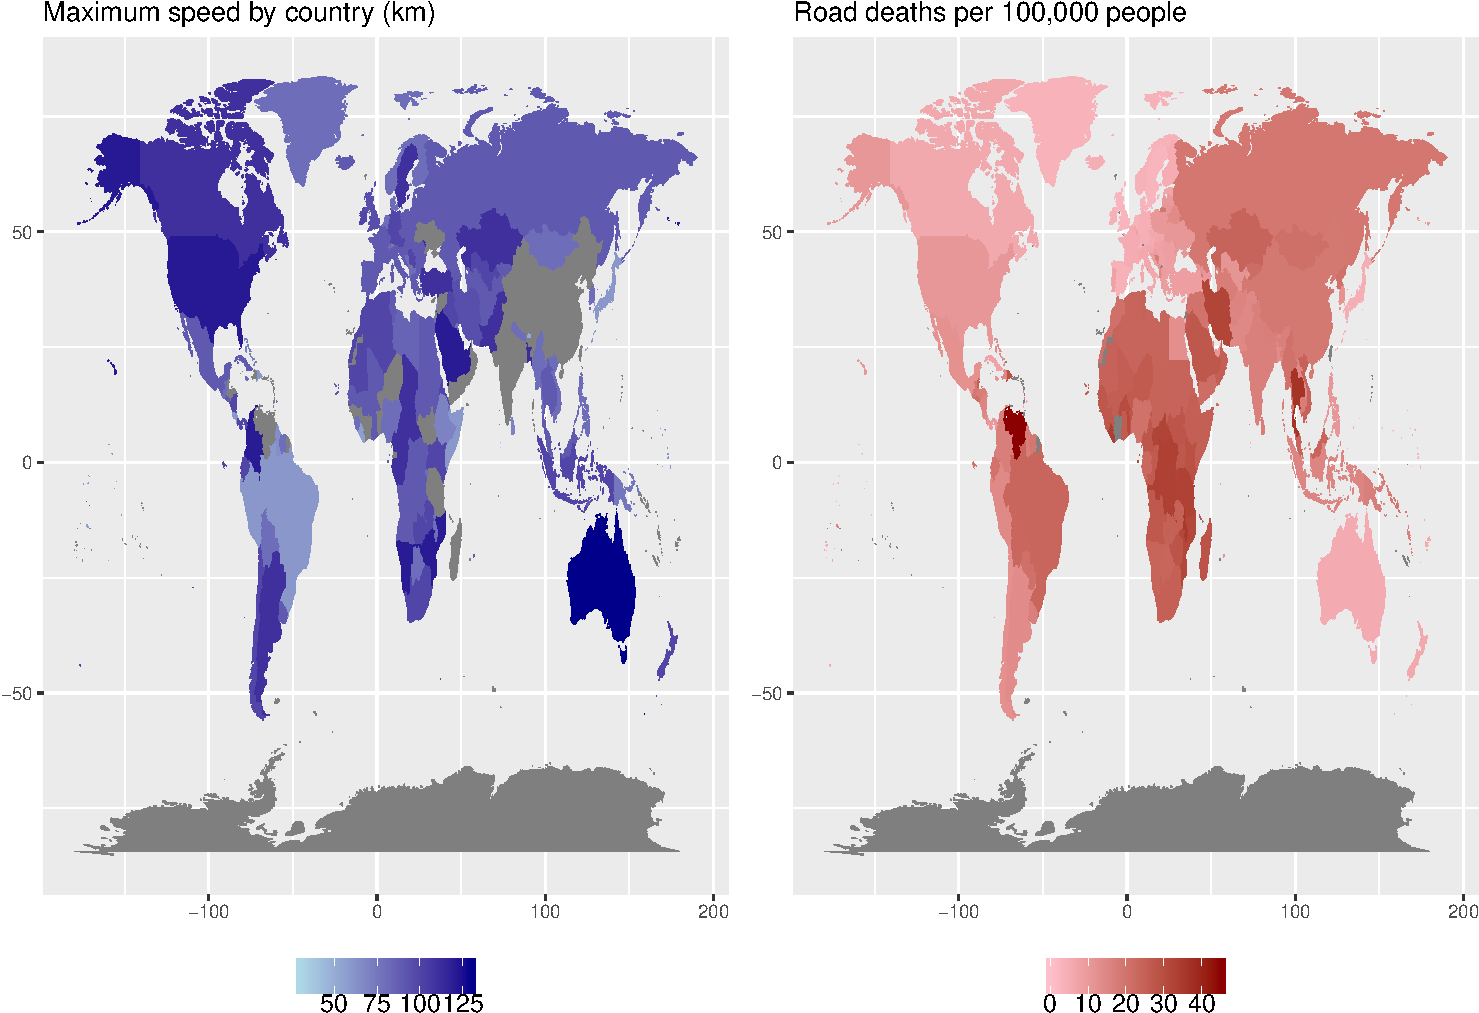
\includegraphics{Slides_files/figure-beamer/unnamed-chunk-22-1} \end{center}

\end{frame}

\begin{frame}{Factor 1: Maps comparing maximum speed limit and rates of
road death by country.}

\begin{center}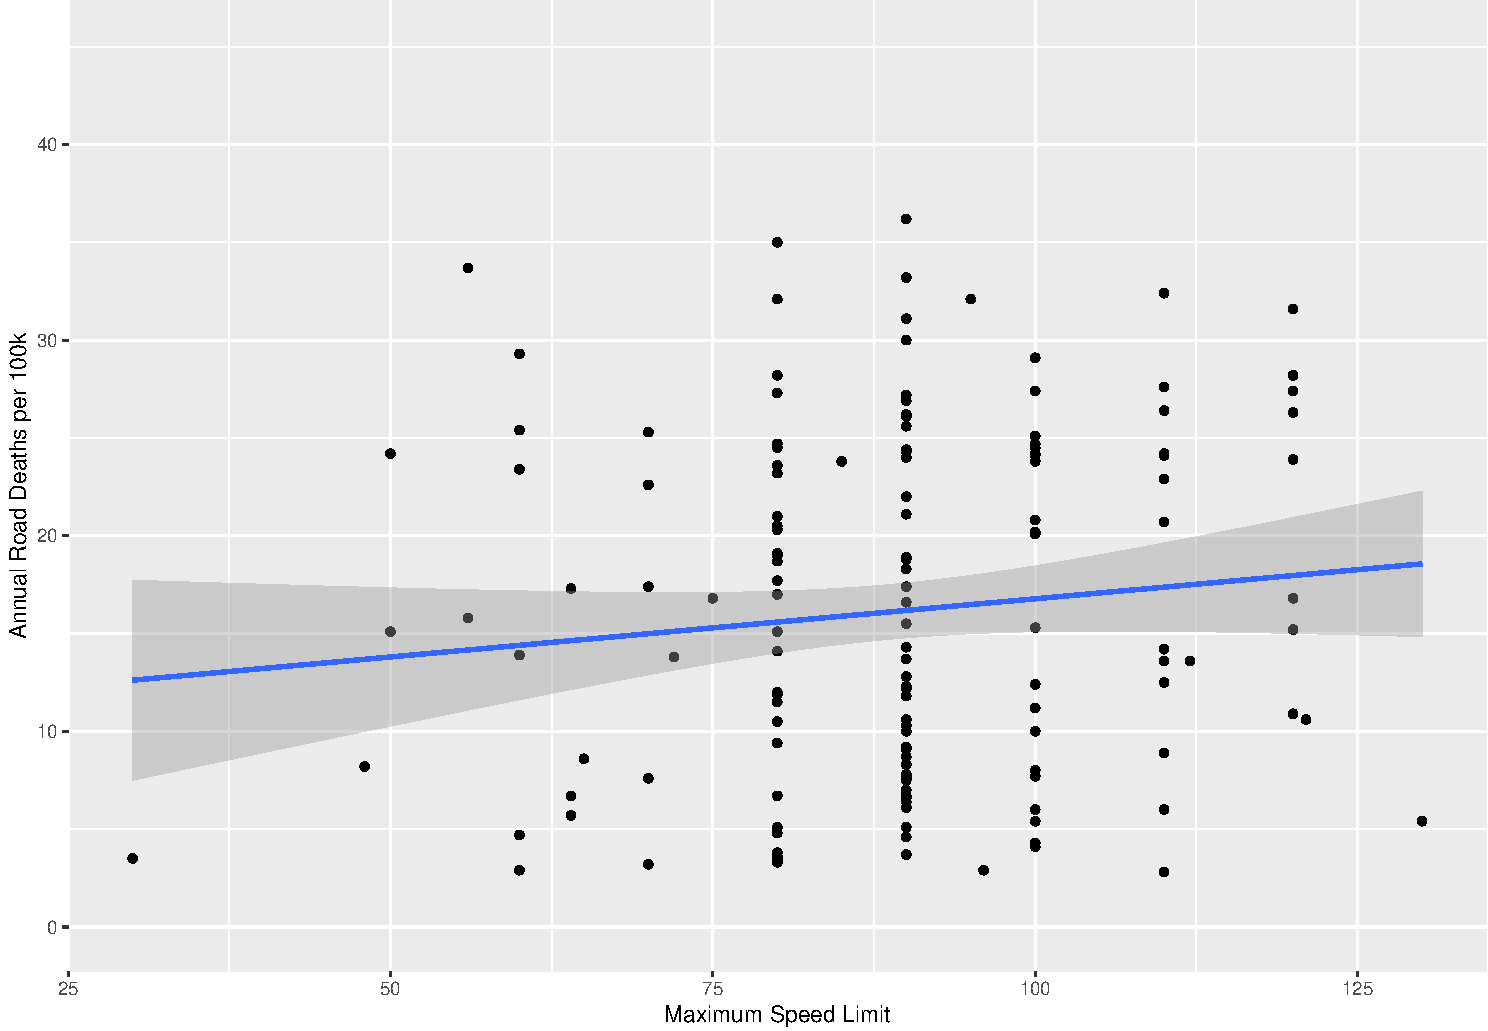
\includegraphics{Slides_files/figure-beamer/unnamed-chunk-23-1} \end{center}

\end{frame}

\begin{frame}{Factor 1: Scatter plot of speed limits versus mortality
rates.}

\begin{center}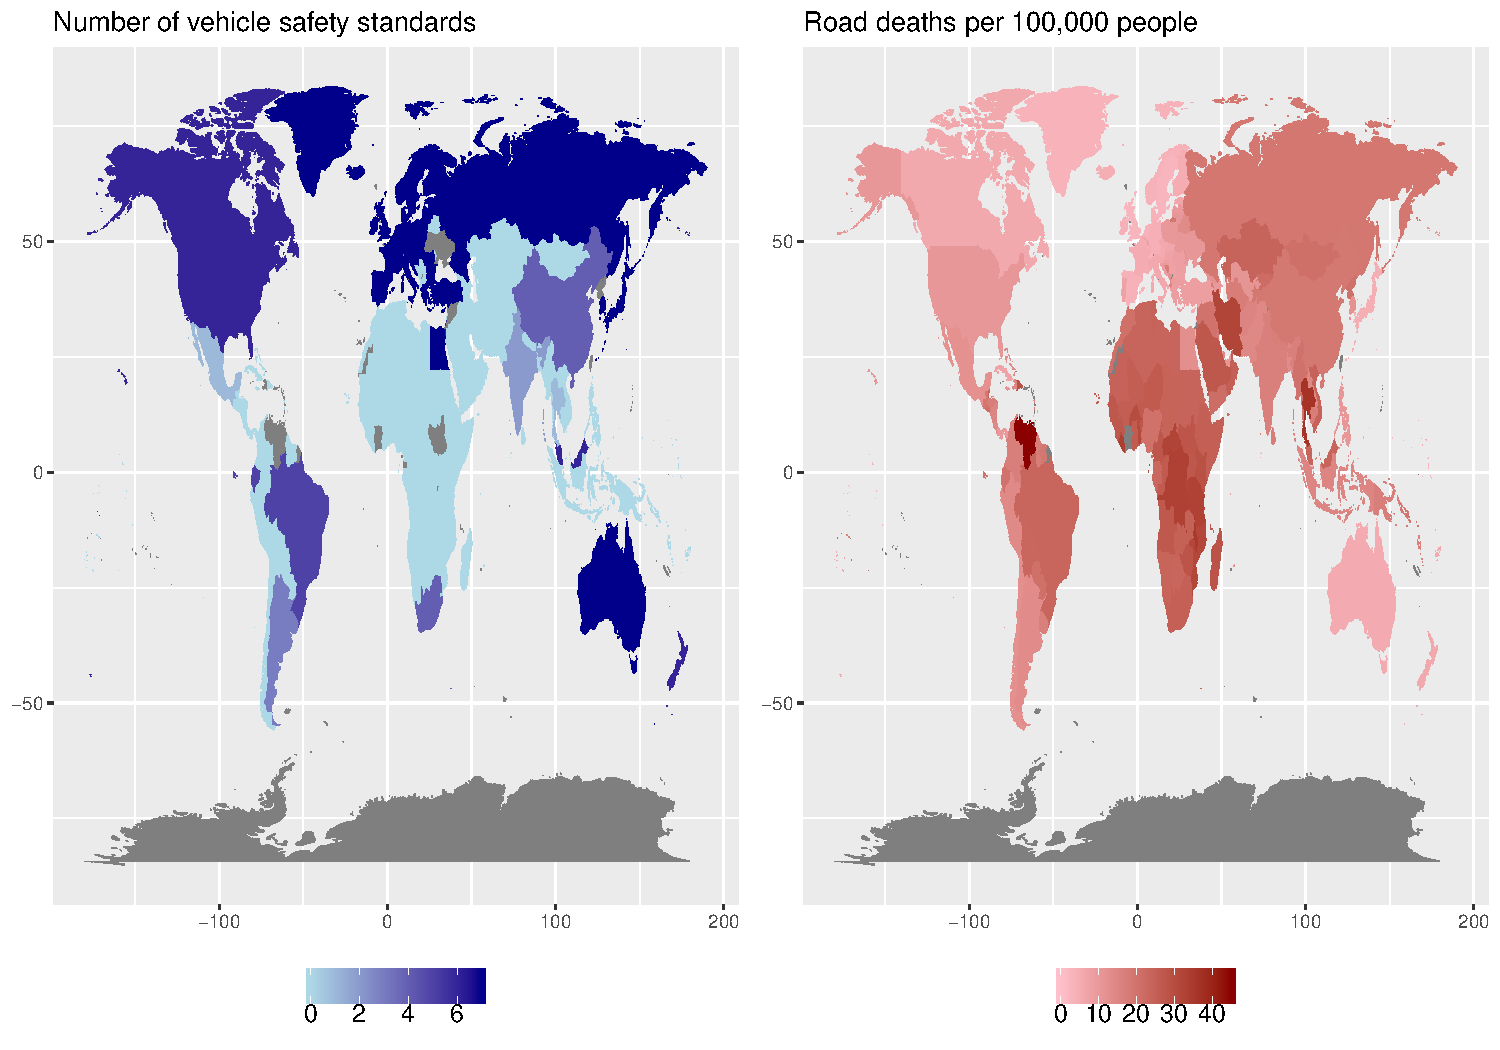
\includegraphics{Slides_files/figure-beamer/unnamed-chunk-24-1} \end{center}

\end{frame}

\begin{frame}{Factor 2: Maps comparing number of vehicle safety
standards and rates of road death by country.}

\begin{center}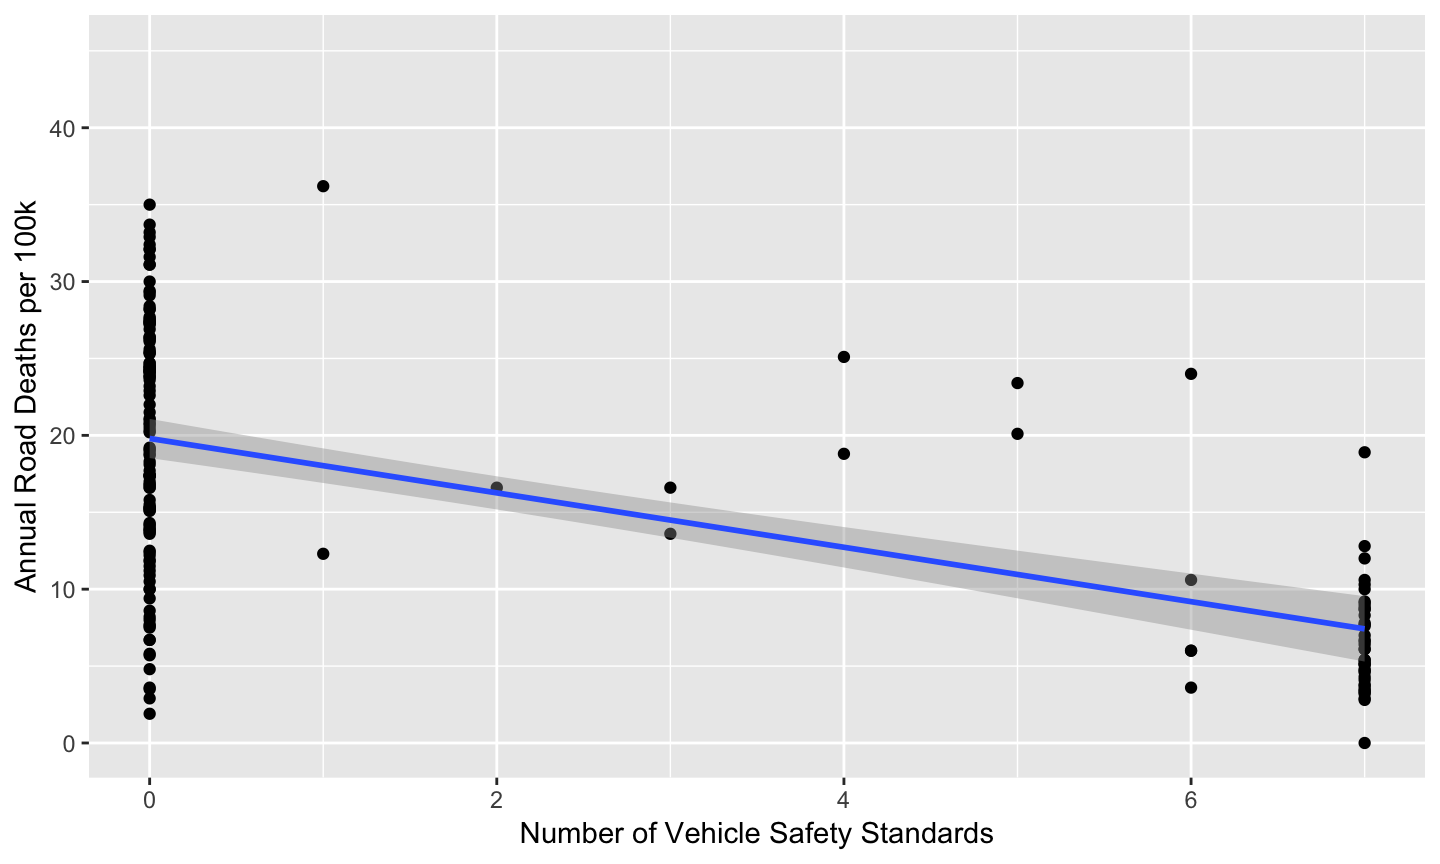
\includegraphics{Slides_files/figure-beamer/unnamed-chunk-25-1} \end{center}

\end{frame}

\begin{frame}{Factor 2: Scatter plot of safety standards versus
mortality rates.}

\begin{center}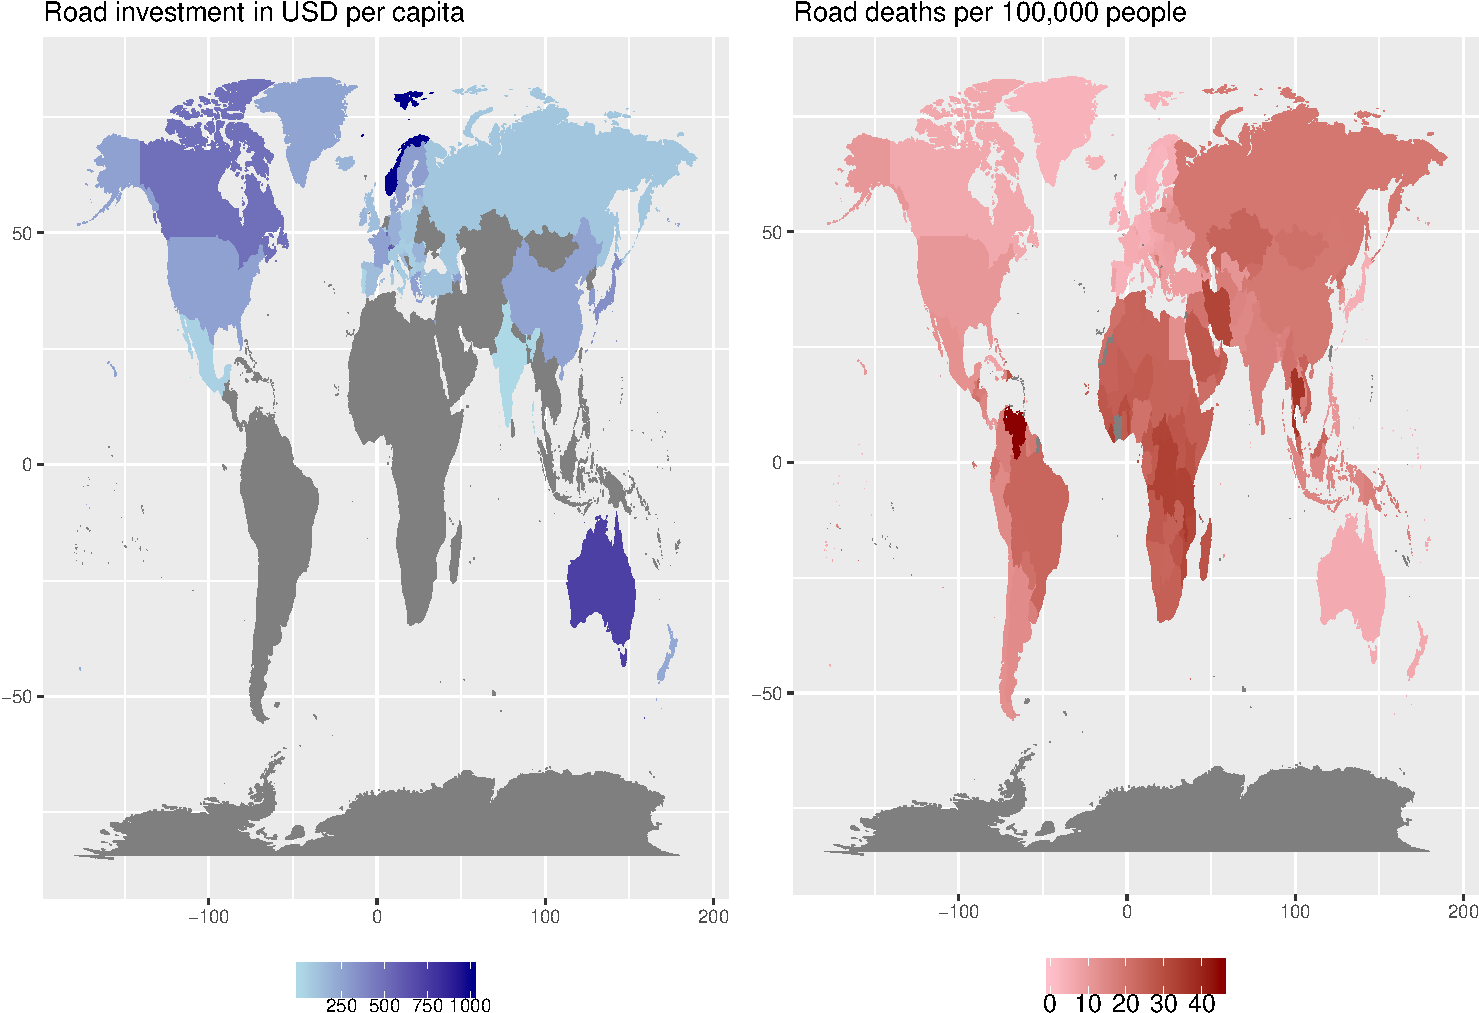
\includegraphics{Slides_files/figure-beamer/unnamed-chunk-26-1} \end{center}

\end{frame}

\begin{frame}{Factor 3: Maps comparing annual infrastructure spending
and rates of road death by country.}

\begin{center}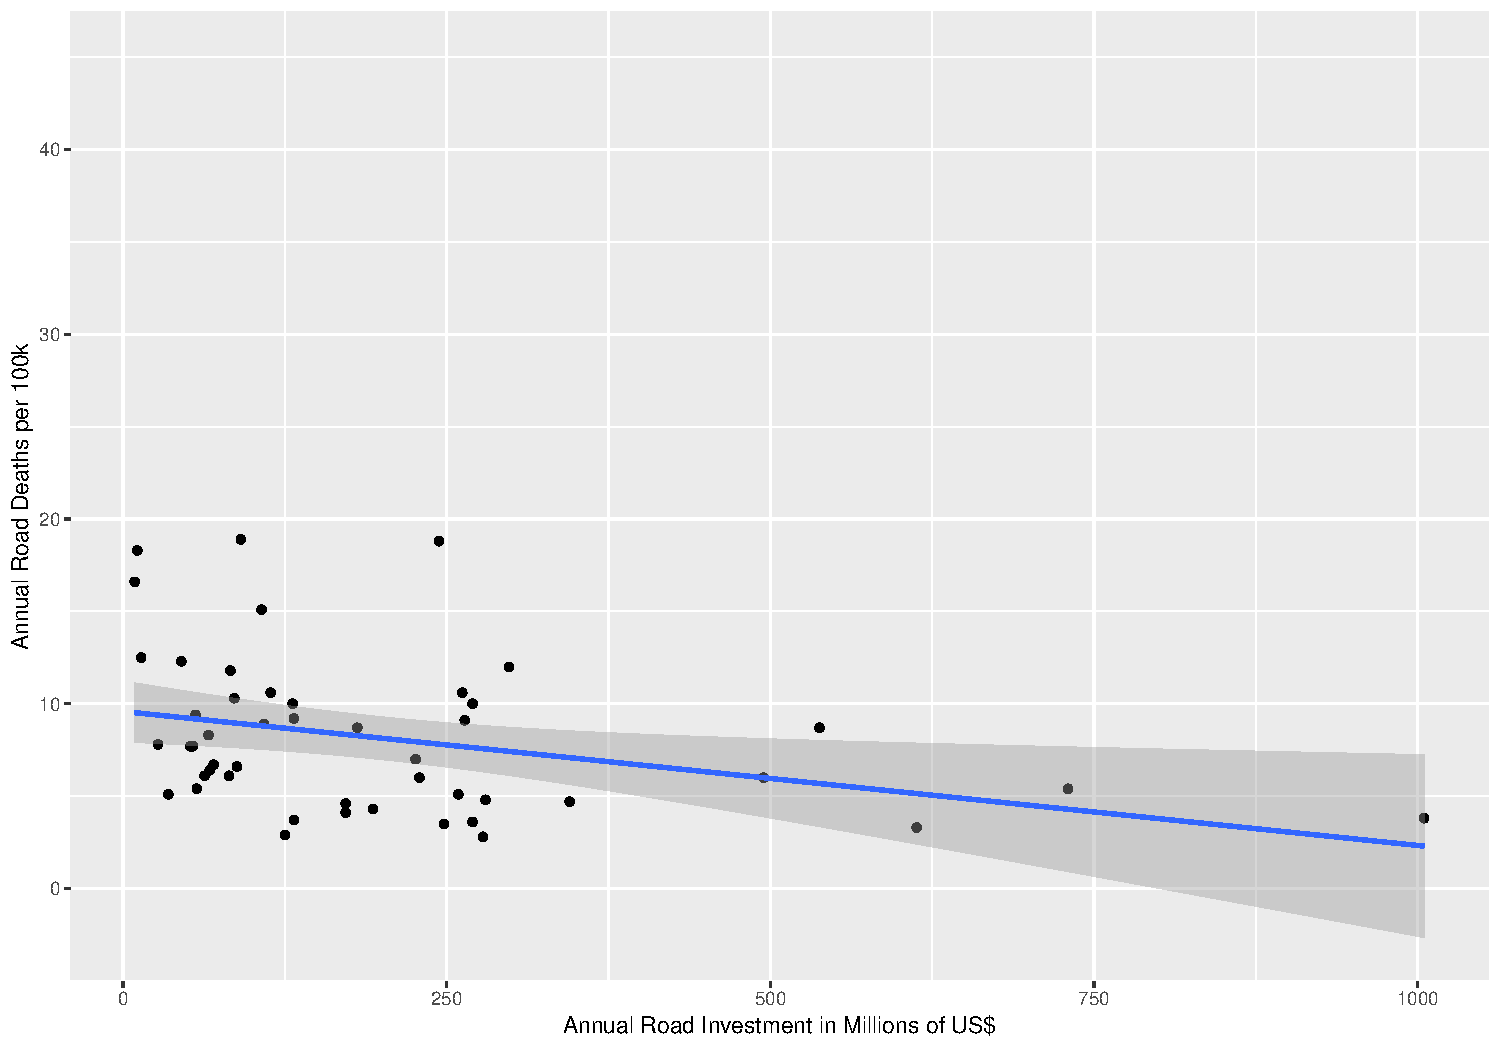
\includegraphics{Slides_files/figure-beamer/unnamed-chunk-27-1} \end{center}

\end{frame}

\begin{frame}{Factor 3: Scatter plot of Infrastructure Spending versus
mortality rates.}

\begin{center}\includegraphics{Slides_files/figure-beamer/unnamed-chunk-28-1} \end{center}

\end{frame}

\begin{frame}{Factor 4: Maps comparing congestion and rates of road
death by country.}

\begin{center}\includegraphics{Slides_files/figure-beamer/unnamed-chunk-29-1} \end{center}

\end{frame}

\begin{frame}{Factor 4: Scatter plot of congestion versus mortality
rates.}

\begin{center}\includegraphics{Slides_files/figure-beamer/unnamed-chunk-30-1} \end{center}

\end{frame}

\begin{frame}{Our interactive application}

\href{https://pelzma.shinyapps.io/interactive_plot/}{Click Here to view
the our interactive application}

\end{frame}

\begin{frame}{}

``You can have data without information, but you cannot have information
without data.''- Daniel Keys Moran

Thank You

\end{frame}

\begin{frame}{Reference}

\begin{itemize}
\tightlist
\item
  World Health Organization,
  \url{http://apps.who.int/gho/data/view.main.51421}\\
\item
  International Transportation Forum, Organization for Economic
  Co-operation and Development \url{https://stats.oecd.org/}
\item
  CIA World Factbook
  \url{https://www.cia.gov/library/publications/the-world-factbook/}
\end{itemize}

\end{frame}

\end{document}
